\documentclass[leqno]{article}
\usepackage{amsmath}
\usepackage{titlesec}
\usepackage{graphicx}
\titleformat{\section}{\normalfont\bfseries\itshape}{\thesection}{0.5em}{}
\begin{document}
\begin{flushright}
Matthew Sicotte\\
Physics 326 Section 01\\
September 11, 2018
\end{flushright}
\begin{center}
	{\large \bf Lab 1: Propagation of Error}
\end{center}
\section*{Introduction:}
When we perform scientific experiments, we often have to take multiple measurements of a certain quantity.  In this case, we need to be able to calculate the error of the average of these measurements so that we can treat it as a single measurement with a higher level of accuracy.  To find the error of the average, we calculate the standard error, which is equal to the standard deviation (found using Eq.(1)) divided by the square root of the number of trials performed, as shown in Eq.(2).  
\begin{equation}
	\sigma=\sqrt{\frac{1}{N-1}\sum_{i=1}^{N} (x_i-\bar{x})^2}
\end{equation}
\begin{equation}
	\sigma_{\bar{x}}=\frac{\sigma}{\sqrt{n}}
\end{equation}\\

Additionally, we often have to determine how the errors for each measurement influence our final results.  To do this, it is necessary to use the propagation of error formula.  Suppose that \{$x_1, x_2, \ldots, x_n$\} is a set of $n$ measurements, with errors of \{$\delta x_1, \delta x_2, \ldots, \delta x_n$\}, and we want to find the error in the value of a variable $q$, which is a function of \{$x_1, x_2, \ldots, x_n$\}.  Then, the error contributed to $q$ from \{$x_1, x_2, \ldots, x_n$\} is found exactly by Eq.(3) and quickly estimated by Eq.(4).  The error contributed to $q$ by a single measured quantiy $a$ is found using Eq.(5). 


\begin{equation}
	\delta q=\sqrt{(\frac{\partial q}{\partial x_1}\delta x_1)^2+(\frac{\partial q}{\partial x_2}\delta x_2)^2+\ldots+(\frac{\partial q}{\partial x_n}\delta x_n)^2}
\end{equation}

\begin{equation}
	\delta q \leq |\frac{\partial q}{\partial x_1}\delta x_1|+|\frac{\partial q}{\partial x_2}\delta x_2|+\ldots + |\frac{\partial q}{\partial x_n}\delta x_n|
\end{equation}
\begin{equation}
	\delta q_a=|\frac{\partial q}{\partial a}\delta a|
\end{equation}
In this lab, we will be using a torsion pendulum to determine the modulus of rigidity for a steel wire.
In this case, the equation for the modulus of rigidity, M, is given by Eq.(6)
\begin{equation}
	M=\frac{32\pi}{3}\frac{Lm(a^2+b^2)}{d^4T^2}
\end{equation}
where $L$ is the length of the wire, $m$ is the mass of the bar, $a$ is the length of the bar, $b$ is the width of the bar, $d$ is the diameter of the wire, and $T$ is the period of the torsion pendulum, all of which are measured.\\\\
The main objective of this lab is to learn about errors in measurement and how they affect our final calculated value.  Additionally, we will be calculating the propagation of error due to each measurement and taking multiple measurements where necessary to reduce our errors.  To do this, we determined the modulus of rigidity of a steel wire using a torsion pendulum.
\section*{Experimental Method:}
This lab consisted of the following apparatus.  A long, thin steel wire was hung from a standard lab stand.  The bottom of the wire was threaded through a small hole in the central vertical axis of a brass bar.  A screw was threaded through a larger hole parallel to the width of the bar to hold the bottom end of the wire in place.\\

\noindent For our measurements, we used a micrometer to measure the width of the block and the diameter of the wire.  To measure the length of the wire, we used a meter ruler with markings every 1 mm.  Digital calipers were used to measure the length of the bar.  Additionally, to measure the mass of the bar, a standard scale was used.  Finally, to measure the period of the torsion pendulum, we used a stopwatch on a cell phone.\\

\noindent For the first part of this lab, we determined the least count of each instrument to get a rough idea of the error of each of our measurements.  As it was very hard to get a very precise measurement of the width of the bar, we took three different measurements, determined the average and the standard error, and then estimated the propagation of error using Eq.(4) and Eq.(6).  By analyzing this result, we found that the largest errors were from our measurements of the diameter of the wire and the period of the torsion pendulum.\\

\noindent For the second part of the lab, we improved the measurements with the largest errors by taking multiple trials and finding their average values nad standard errors.  For each of these measurements, the standard deviation of the mean, or standard error, is considered to be the appropriate error as we performed many trials.  For the measurements that were stable and did not have any significant variation from trial to trial, we used the least count of the instrument as our error.\\

\noindent Finally, to find the modulus of rigidity, we used Eq.(6) to find the average value and Eq. (3) and Eq. (6) to find the error.  
\section*{First Part Results:}
In the first part of this lab, we took one measurement of each quantity and determined the least count and stability of each measurement.  Table 1.1 shows our measurements for the least count and stability of our initial measurements.\\\\
\textbf{Table 1.1}\\\\
\begin{tabular}{|c|c|c|c|c|c|c|}
	\hline
	Measurement & L (m)& m (kg)& a (m)& b (m)& d (m)& T (s)\\
	\hline
	Least count & $1 \times 10^{-3}$ & $1\times 10^{-4}$ & $1 \times 10^{-4}$ & $1 \times 10^{-6}$ & $1 \times 10^{-6}$ & $0.1$\\
	\hline
	Stable & Yes & Yes & Yes & No & Yes & Yes\\
	\hline
\end{tabular}
\begin{flushleft}
\textit{\small Table 1.1: Least count and stability of initial measurements.}
\end{flushleft}
Since the measurement for b was not stable, we took three measurements for b (shown in Table 1.2) and calculated the average and standard error for these measurements (shown in Table 1.3).\\\\
\textbf{Table 1.2}\\\\
\begin{tabular}{|c|c|c|c|}
	\hline
	Trial $m$ & 1 & 2 & 3\\
	\hline
	$b (m)$ & $1.9066 \times 10^{-2}$ & $1.9006 \times 10^{-2}$ & $1.9023 \times 10^{-2}$\\
	\hline
\end{tabular}
\begin{flushleft}
\textit{\small Table 1.2: Measurements of the width of the bar, b.}
\end{flushleft}
\textbf{Table 1.3}\\\\
\begin{tabular}{|c|c|}
	\hline
	Average $\bar{b}$ (m) & Standard Error $\sigma_{\bar{b}}$ (m)\\
	\hline
	19.03 & 0.02\\
	\hline
\end{tabular}
\begin{flushleft}
\textit{\small Table 1.3: Calculated average value and standard error for b (using Eq.(2)).}
\end{flushleft}
Upon analyzing the stability and uncertainty of our measurements, we obtained the following initial values, as shown in Table 1.4.\\\\
\textbf{Table 1.4}\\\\
\begin{tabular}{c|l}
Variable & Value\\
L & $(8.29\pm0.01)\times10^{-1}$ m\\
m & $(2.360\pm0.001)\times 10^{-1}$ kg\\
a & $(1.144\pm0.001)\times10^{-1}$ m\\
b & $(1.903\pm0.002)\times10^{-2}$ m\\
d & $(4.77\pm0.01)\times10^{-4}$ m\\
T & $4.0 \pm 0.1$ s\\
\end{tabular}
\begin{flushleft}
\textit{\small Table 1.4: Initial values and errors for the six measured quantities.}
\end{flushleft}
Then, by using Eq.(5) for each of our measured quantities, we estimated the error contributed to our desired quantity, M, from each measurement.
By performing the required differentiation of M, we determined the formulas for the error contributed by each quantity, as shown in Table 1.5.\newpage
\textbf{Table 1.5}\\\\
\begin{tabular}{|c|c|c|c|}
	\hline
	Quantity & L & m & a\\
	\hline
	Error due to Measurement& $\frac{32\pi}{3}\frac{m(a^2+b^2)}{d^4 T^2}\delta L$ & $\frac{32\pi}{3}\frac{L(a^2+b^2)}{d^4 T^2}\delta m$ & $\frac{32\pi}{3}\frac{2Lma}{d^4 T^2}\delta a$  \\
\hline
Error due to Measurement (Pa)& $1.3\times10^8$ & $3\times10^7$ & $1.8\times10^8$\\
\hline
\end{tabular}\\\\\\
\begin{tabular}{|c|c|c|c|}
\hline
Quantity & b & d & T\\
\hline
Error due to Measurement & $\frac{32\pi}{3}\frac{2Lmb}{d^4 T^2}\delta b$ & $\frac{32\pi}{3}\frac{4Lm(a^2+b^2)}{d^5 T^2}\delta d$ & $\frac{32\pi}{3}\frac{2Lm(a^2+b^2)}{d^4 T^3}\delta T$\\
\hline
Error due to Measurement (Pa)& $6\times10^6$ & $9\times10^8$ & $5\times10^9$\\
\hline
\end{tabular}
\begin{flushleft}
\textit{\small Table 1.5: Equations and values for the error of M due to our measurement of each quantity.  All equations were directly found using Eq. (5) by partially differentiating the expression for M (Eq. (6)) with respect to the appropriate variable and multiplying by the appropriate error (shown in table 1.4).}
\end{flushleft}
Using Eq. (4), we obtained a total error of $7 \times 10^9$ Pa, or 7 GPa.\\
In comparison, our estimated value for the modulus of rigidity, M, was 106 GPa, or $1.06\times10^{11}$ Pa.\\\\
Based on the analysis of these errors, the most important quantities to be measured again multiple times were the diameter of the wire and the period of the torsion pendulum.  The period, T, was especially important to measure multiple times because our measurements may have been influenced by our reaction times as well as other variables relating to each trial such as air resistance.
\section*{Second Part Results:}
Upon determining the quantities to re-measure, we took 24 different measurements for the period, T, and 6 measurements at different points of the wire for the diameter, d.  All other quantities measured appeared to be stable, so we used our values from the first part of the lab.  The average value  and associated error of each measured quantity is shown in Table 2.1.\\\\
\textbf{Table 2.1}\\\\
\begin{tabular}{c|c}
	Quantity & Value\\
	\hline
	L & $(8.29\pm0.01)\times 10^{-1}$ m\\
	m & $(2.360\pm0.001)\times 10^{-1}$ kg\\
	a & $(1.144\pm0.001)\times 10^{-1}$ m\\
	b & $(1.9032\pm0.0018)\times10^{-2}$ m\\
	d & $(5.072\pm0.005)\times 10^{-4}$ m\\
	T & $(3.76\pm0.03)$ s\\
\end{tabular}
\begin{flushleft}
\textit{\small Table 2.1: Final values for the average value and error of each measured quantity.  For l, m, and a, due to stable measurements, the error is the least count of the instrument used.  For all other values, the error was calculated using Eq. (2).}
\end{flushleft}
\section*{Analysis:}
Using Eq. (3) and Eq. (6), we obtained a value for M of $(9.4\pm0.2)\times10^{10}$ Pa, which is $94\pm2$ GPa.  This is about a 2-percent error, well within our target of 5 percent.  As a comparison, the handbook value for the modulus of rigidity for steel is generally about 80 GPa, but it varies from 70 to 90 GPa.  Thus, our measurements for M are close to the range of accepted values, but there were likely some significant sources of error beyond our measurements.
\section*{Conclusions:}
In conclusion, this lab helped us learn about errors in measured quantities and the propagation of error.  Although the most commonly stated modulus of rigidity of steel is 80 GPa, which is about 7 standard errors lesss than our experimental value, there is significant variation in different types of steel.\\\\
 Additionally, there were also many other possible sources of error in our lab.  For example, there was a hole in the bar that housed a screw made of a different metal.  This could have significantly altered the bar's moment of inertia, which would have made Eq. (6) slightly inaccurate.  Also, the brass bar wobbled slightly as it was spinning, and the wire was of varying thickness, which could have also made Eq. (6) inaccurate.  However, despite these errors, we still got a fairly accurate value for the modulus of rigidity of our steel wire.
\newpage
\section*{Appendix A: Raw Data for Part 1:}
\noindent
\textbf{Table A.1}\\\\
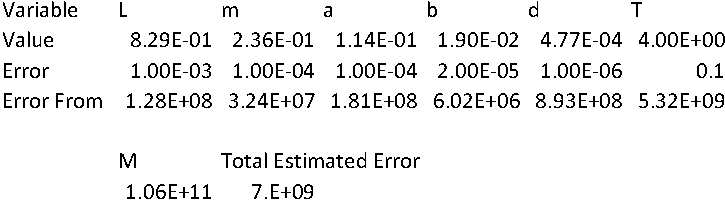
\includegraphics[width=\linewidth]{lab1dataa-crop}\\\\
\textit{\small Table A.1: Excel spreadsheet with measurements from part 1.}
\newpage
\textbf{Table A.2}\\
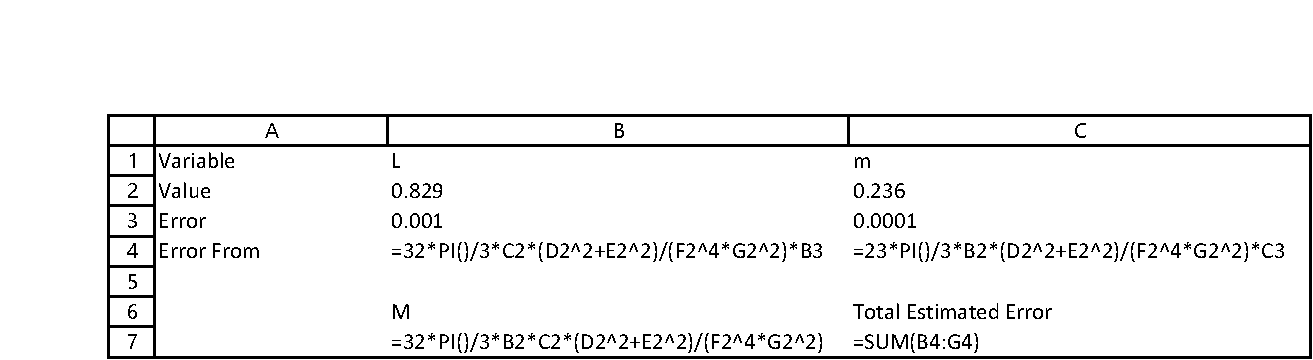
\includegraphics[width=\linewidth]{lab1dataaf1-crop}
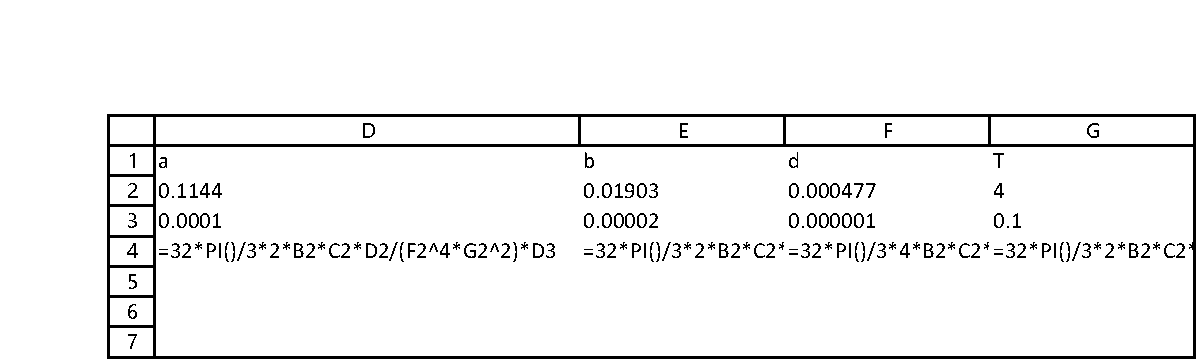
\includegraphics[width=\linewidth]{lab1dataaf2-crop}\\\\
\textit{\small Table A.2: Excel spreadsheet with formulas from part 1.}
\newpage
\section*{Appendix B: Raw Data for Part 2:}
\noindent
\textbf{Table B.1}\\\\
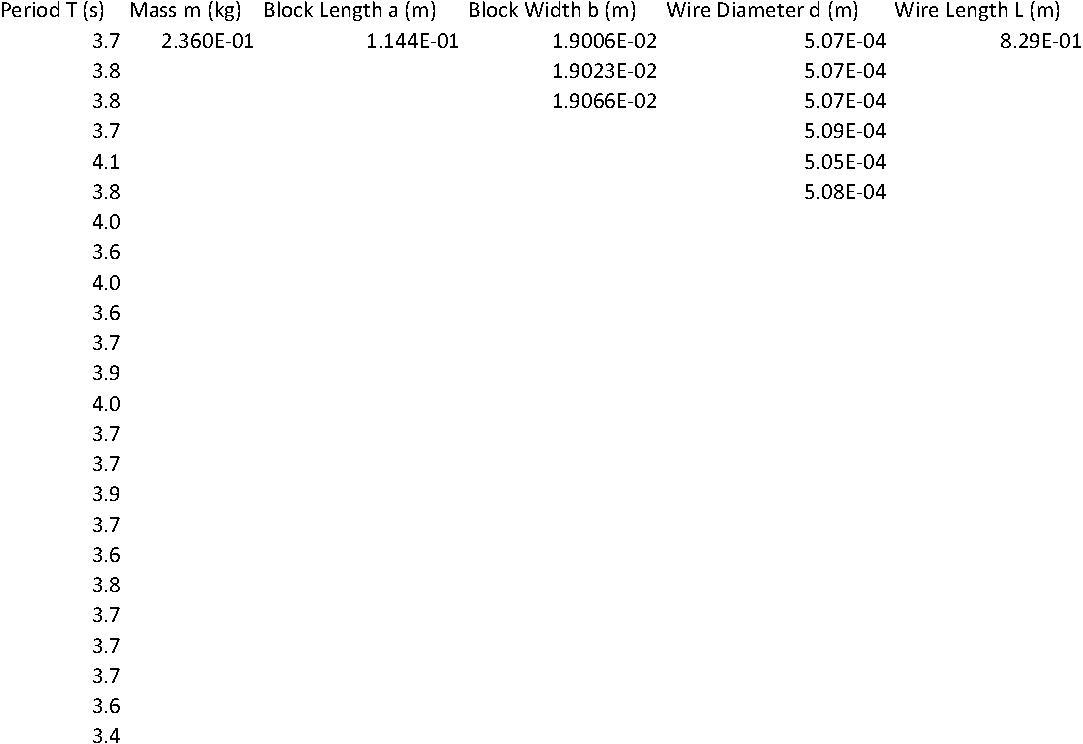
\includegraphics[width=\linewidth]{lab1datab-crop}\\\\
\textit{\small Table B.1: Excel spreadsheet with trial-by-trial measurements from part 2.}
\newpage
\noindent\textbf{Table B.2}\\\\
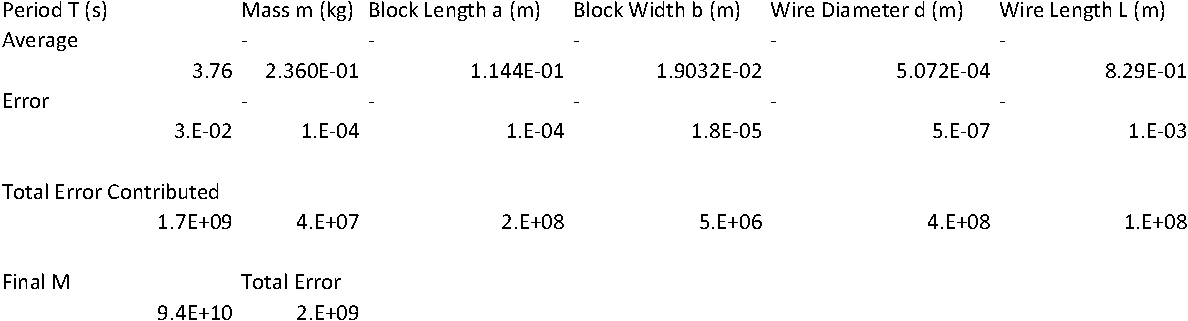
\includegraphics[width=\linewidth]{lab1datac-crop}\\\\
\textit{\small Table B.2: Excel spreadsheet with final measurements from part 2.}
\newpage
\textbf{Table B.3}\\
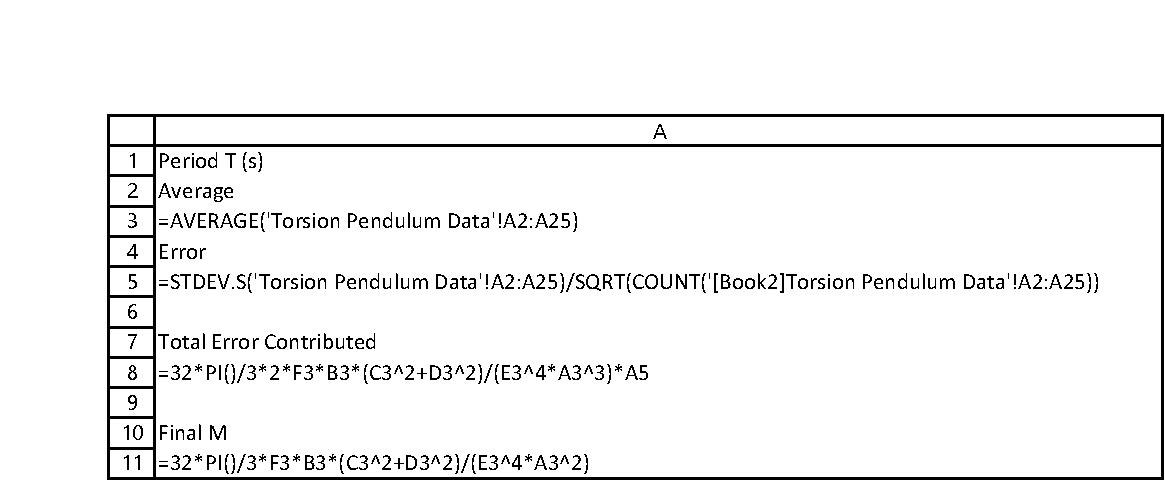
\includegraphics[width=\linewidth]{lab1datacf1-crop}
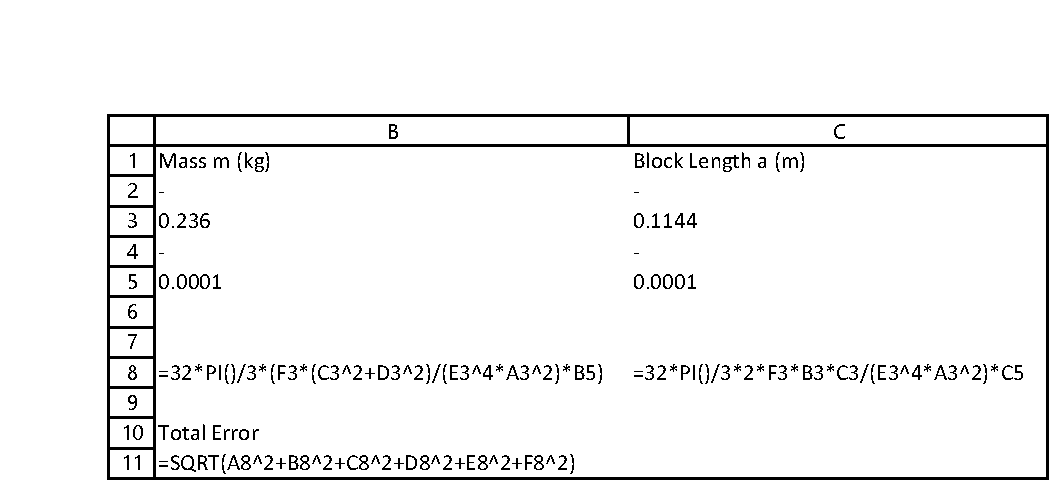
\includegraphics[width=\linewidth]{lab1datacf2-crop}
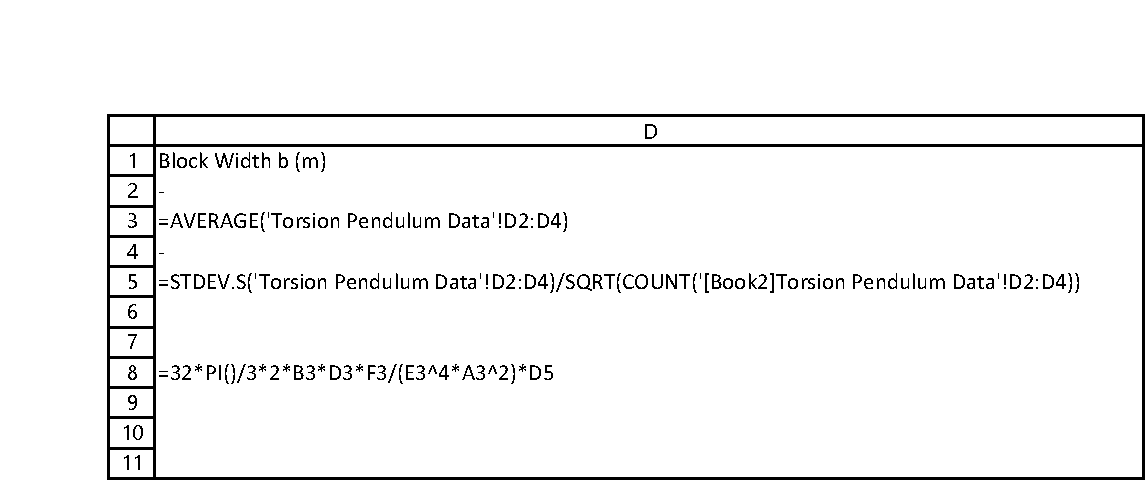
\includegraphics[width=\linewidth]{lab1datacf3-crop}
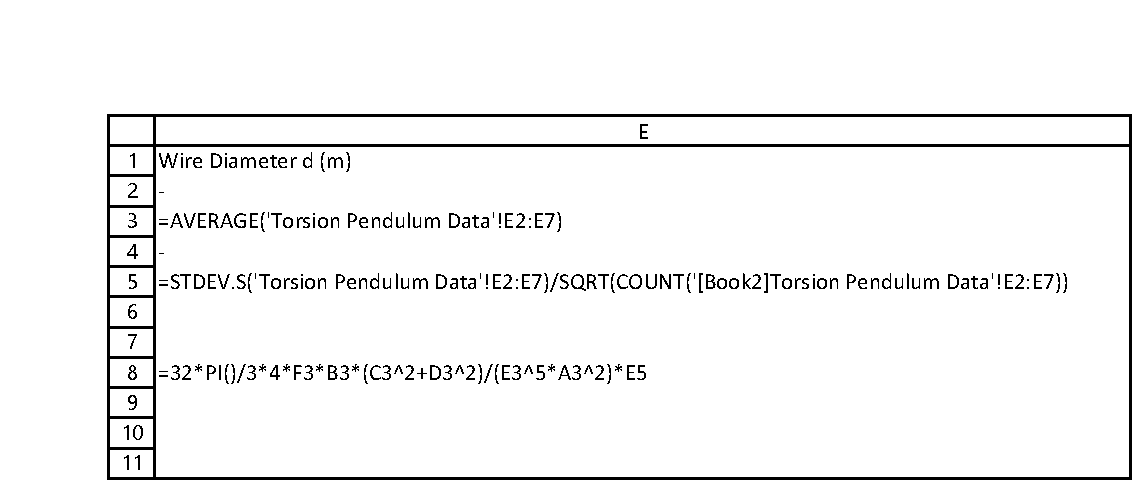
\includegraphics[width=\linewidth]{lab1datacf4-crop}
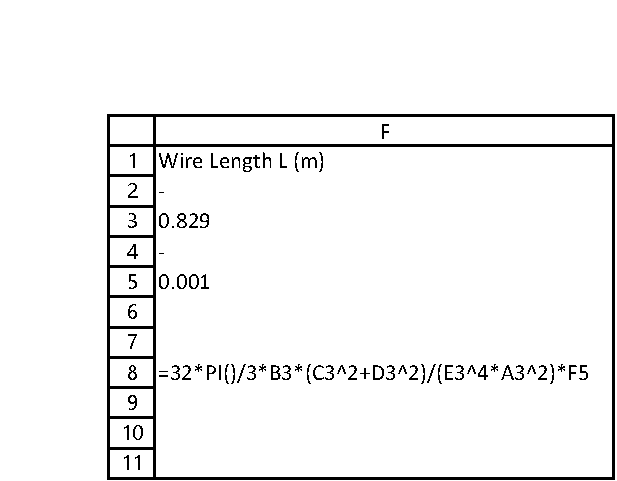
\includegraphics[width=0.6\linewidth]{lab1datacf5-crop}\\\\
\textit{\small Table B.3: Excel spreadsheet with formulas from part 2.}
\end{document}
